\documentclass[10pt,letterpaper]{article}
\usepackage[top=0.85in,left=2.75in,footskip=0.75in]{geometry}

\usepackage{changepage}

\usepackage[utf8]{inputenc}

\usepackage{textcomp,marvosym}

\usepackage{fixltx2e}

\usepackage{amsmath,amssymb}

\usepackage{cite}

\usepackage{nameref,hyperref}

\usepackage[right]{lineno}

\usepackage{microtype}
\DisableLigatures[f]{encoding = *, family = * }

\usepackage{rotating}

\raggedright
\setlength{\parindent}{0.5cm}
\textwidth 5.25in 
\textheight 8.75in

\usepackage[aboveskip=1pt,labelfont=bf,labelsep=period,justification=raggedright,singlelinecheck=off]{caption}

% ==== begin added by me =====
\usepackage{svg}

\usepackage{float}

\usepackage[status=draft]{fixme}
\fxuselayouts{footnote,nomargin}

\usepackage{xstring}
\newcommand{\fillin}[1]{
    \IfEqCase{#1}{%
        {short}{\_}%
        {long}{\_\_\_\_\_}%
    }[\PackageError{fillin}{Undefined option to fillin: #1}{}]
}

\usepackage{nameref}
% ==== end added by me =====

\bibliographystyle{plos2015}

\makeatletter
\renewcommand{\@biblabel}[1]{\quad#1.}
\makeatother

\date{}

\usepackage{lastpage,fancyhdr,graphicx}
\usepackage{epstopdf}
\pagestyle{myheadings}
\pagestyle{fancy}
\fancyhf{}
\lhead{
\includegraphics[width=2.0in]{PLOS-Submission.eps}}
\rfoot{\thepage/\pageref{LastPage}}
\renewcommand{\footrule}{\hrule height 2pt \vspace{2mm}}
\fancyheadoffset[L]{2.25in}
\fancyfootoffset[L]{2.25in}
\lfoot{\sf PLOS}

\newcommand{\lorem}{{\bf LOREM}}
\newcommand{\ipsum}{{\bf IPSUM}}

\begin{document}
\vspace*{0.35in}

% Title must be 250 characters or less.
% Please capitalize all terms in the title except conjunctions, prepositions, and articles.
\begin{flushleft}
{\Large
\textbf\newline{Applications of Machine Learning to Automated CFU Counting - Submission to PLOS Journals}
}
\newline
% Insert author names, affiliations and corresponding author email (do not include titles, positions, or degrees).
\\
Shea Conlon\textsuperscript{1} sheaconlon@berkeley.edu,
Will Ludington\textsuperscript{2} will.ludington@berkeley.edu
\\
\bigskip
\bf{1} Department of Molecular and Cell Biology, University of California at Berkeley, Berkeley, CA, USA
\\
\bf{2} Department of Computer Science, University of California at Berkeley, Berkeley, CA, USA
\\
\bigskip
\end{flushleft}
% Please keep the abstract below 300 words
\section*{Abstract}
    Counting colony-forming units (CFUs) on plates of growth medium is a necessary task in many microbiology experiments. Manual CFU counting has multiple drawbacks. First, its high cost in man-hours makes any experiment requiring large-volume CFU counting infeasible. Second, people may produce inconsistent counts, leading to poor data quality. This paper proposes automating CFU counting using machine learning approaches. Specifically, it demonstrates the use of deep convolutional neural networks to count via image segmentation and the use of support vector machines to count via image classification. It shows that these approaches improve the human cost and consistency of CFU counting and can generalize to different laboratory conditions.

\linenumbers

\section*{Introduction}
    Counting colony-forming units (CFUs) on plates of growth medium is a necessary task in many microbiology experiments, such as \fillin{long}. Manual CFU counting has the following drawbacks.

    \begin{enumerate}
        \item \textit{Lack of Scalability.}
            In our experience, it takes an average of $\fillin{short}$ minutes to manually count a single plate of $\fillin{short}$-$\fillin{short}$ CFUs. This high cost in man-hours makes any experiment requiring large-volume CFU counting infeasible.

            For example, suppose you wanted to examine the interactive effect of two substances on the growth of a particular bacterial strain. You could apply perpendicular concentration gradients of the two substances on a $96$-well plate. Counting even a single $96$-well plate would require counting $96$ wells, so you would be restricted to a small number of them.
    
            In another example, suppose you wanted to examine colony growth over time. You could take a video of a plate and count the number of CFUs present at time $0$, time $30$ minutes, etc. Tracking the growth of even a single plate over $24$ hours of growth would require $48$ CFU counts.
        
        \item \textit{Lack of Consistency.}
            In our experience, CFU counts produced by different people differ significantly. It is then desirable that for a given set of counts, either one person should do all of them or two people should replicate all of them. The first solution can cause a bottleneck in the experimental pipeline and contribute to the lack of scalability above. The second solution wastes time that could be spent doing better things.
    \end{enumerate}
    
    \paragraph*{Related Work.}
        Related work in this area has focused on the segmentation of organs in biomedical images \cite{Novikov, Ronneberger} and cells in microscope images \cite{Valen}. Some has addressed CFU counting, but in the clinical laboratory setting, where conditions are tightly controlled and there are large volumes of data available \cite{Ferrari}. This paper applies the core model\fxnote{Tune Valen et al.'s architecture specifically for this use case.} of \cite{Valen} to CFU counting in the scientific laboratory, where conditions vary widely and data is not readily available. It then analyzes the model's ability to generalize to new conditions and adds measures to make the model reusable by other labs with minimal tuning. Finally, it presents an alternative model for CFU counting that is faster to train and use, along with measures for handling its decreased accuracy.
    
    \paragraph*{Organization.}
        \textit{\nameref{ssec:datasets}} describes the datasets used in our experiments. Section \textit{\nameref{ssec:dcnn}} describes the methodology behind the deep convolutional neural network used for counting CFUs via image segmentation. Section \textit{\nameref{ssec:svm}} describes the methodology behind the support vector machine used for counting CFUs via image classification. Sections \textit{\nameref{ssec:dcnn_results}} and \textit{\nameref{ssec:svm_results}} test the speed, accuracy, and generalization ability of both models.

\section*{Materials and Methods}
    \subsection*{Datasets} \label{ssec:datasets}
        \paragraph*{Image Masks.}
            Going forward, we will refer to "masks" of images. A mask $M$ for condition $c$ of an image $I$ is itself an image of the same dimensions as $I$. $M$'s pixel at $(x, y)$ is black if $c$ is true of $I$'s pixel at $(x, y)$ and white otherwise. For example, in the inside-a-CFU mask for a plate image, the mask's pixel at $(x, y)$ is black if the plate's pixel at $(x, y)$ is inside a CFU and white if it is outside all CFUs.

        \paragraph*{\texttt{easy\_masked} Dataset}
            This dataset consists of $2$ plate images, their masks, and their counts. The masks mark the pixels that are inside a CFU, on the edge of some CFU(s), and outside all CFUs. The plate images were captured with a typical smartphone ($2448px \times 3264px$, RGB) and no special setup. The masks were drawn by hand using Adobe Photoshop and a graphics tablet. The counts were collected according to the usual practices of the group. One example can be seen in Fig.~\ref{easy-masked}. This dataset is used for training the DCNN.

            \begin{figure}[h]
                \graphicspath{{results/preprocess_masked/figures/original/}}
                \includegraphics[width=0.2\textwidth]{easy_0_image}
                
\includegraphics[width=0.2\textwidth]{easy_0_inside}
                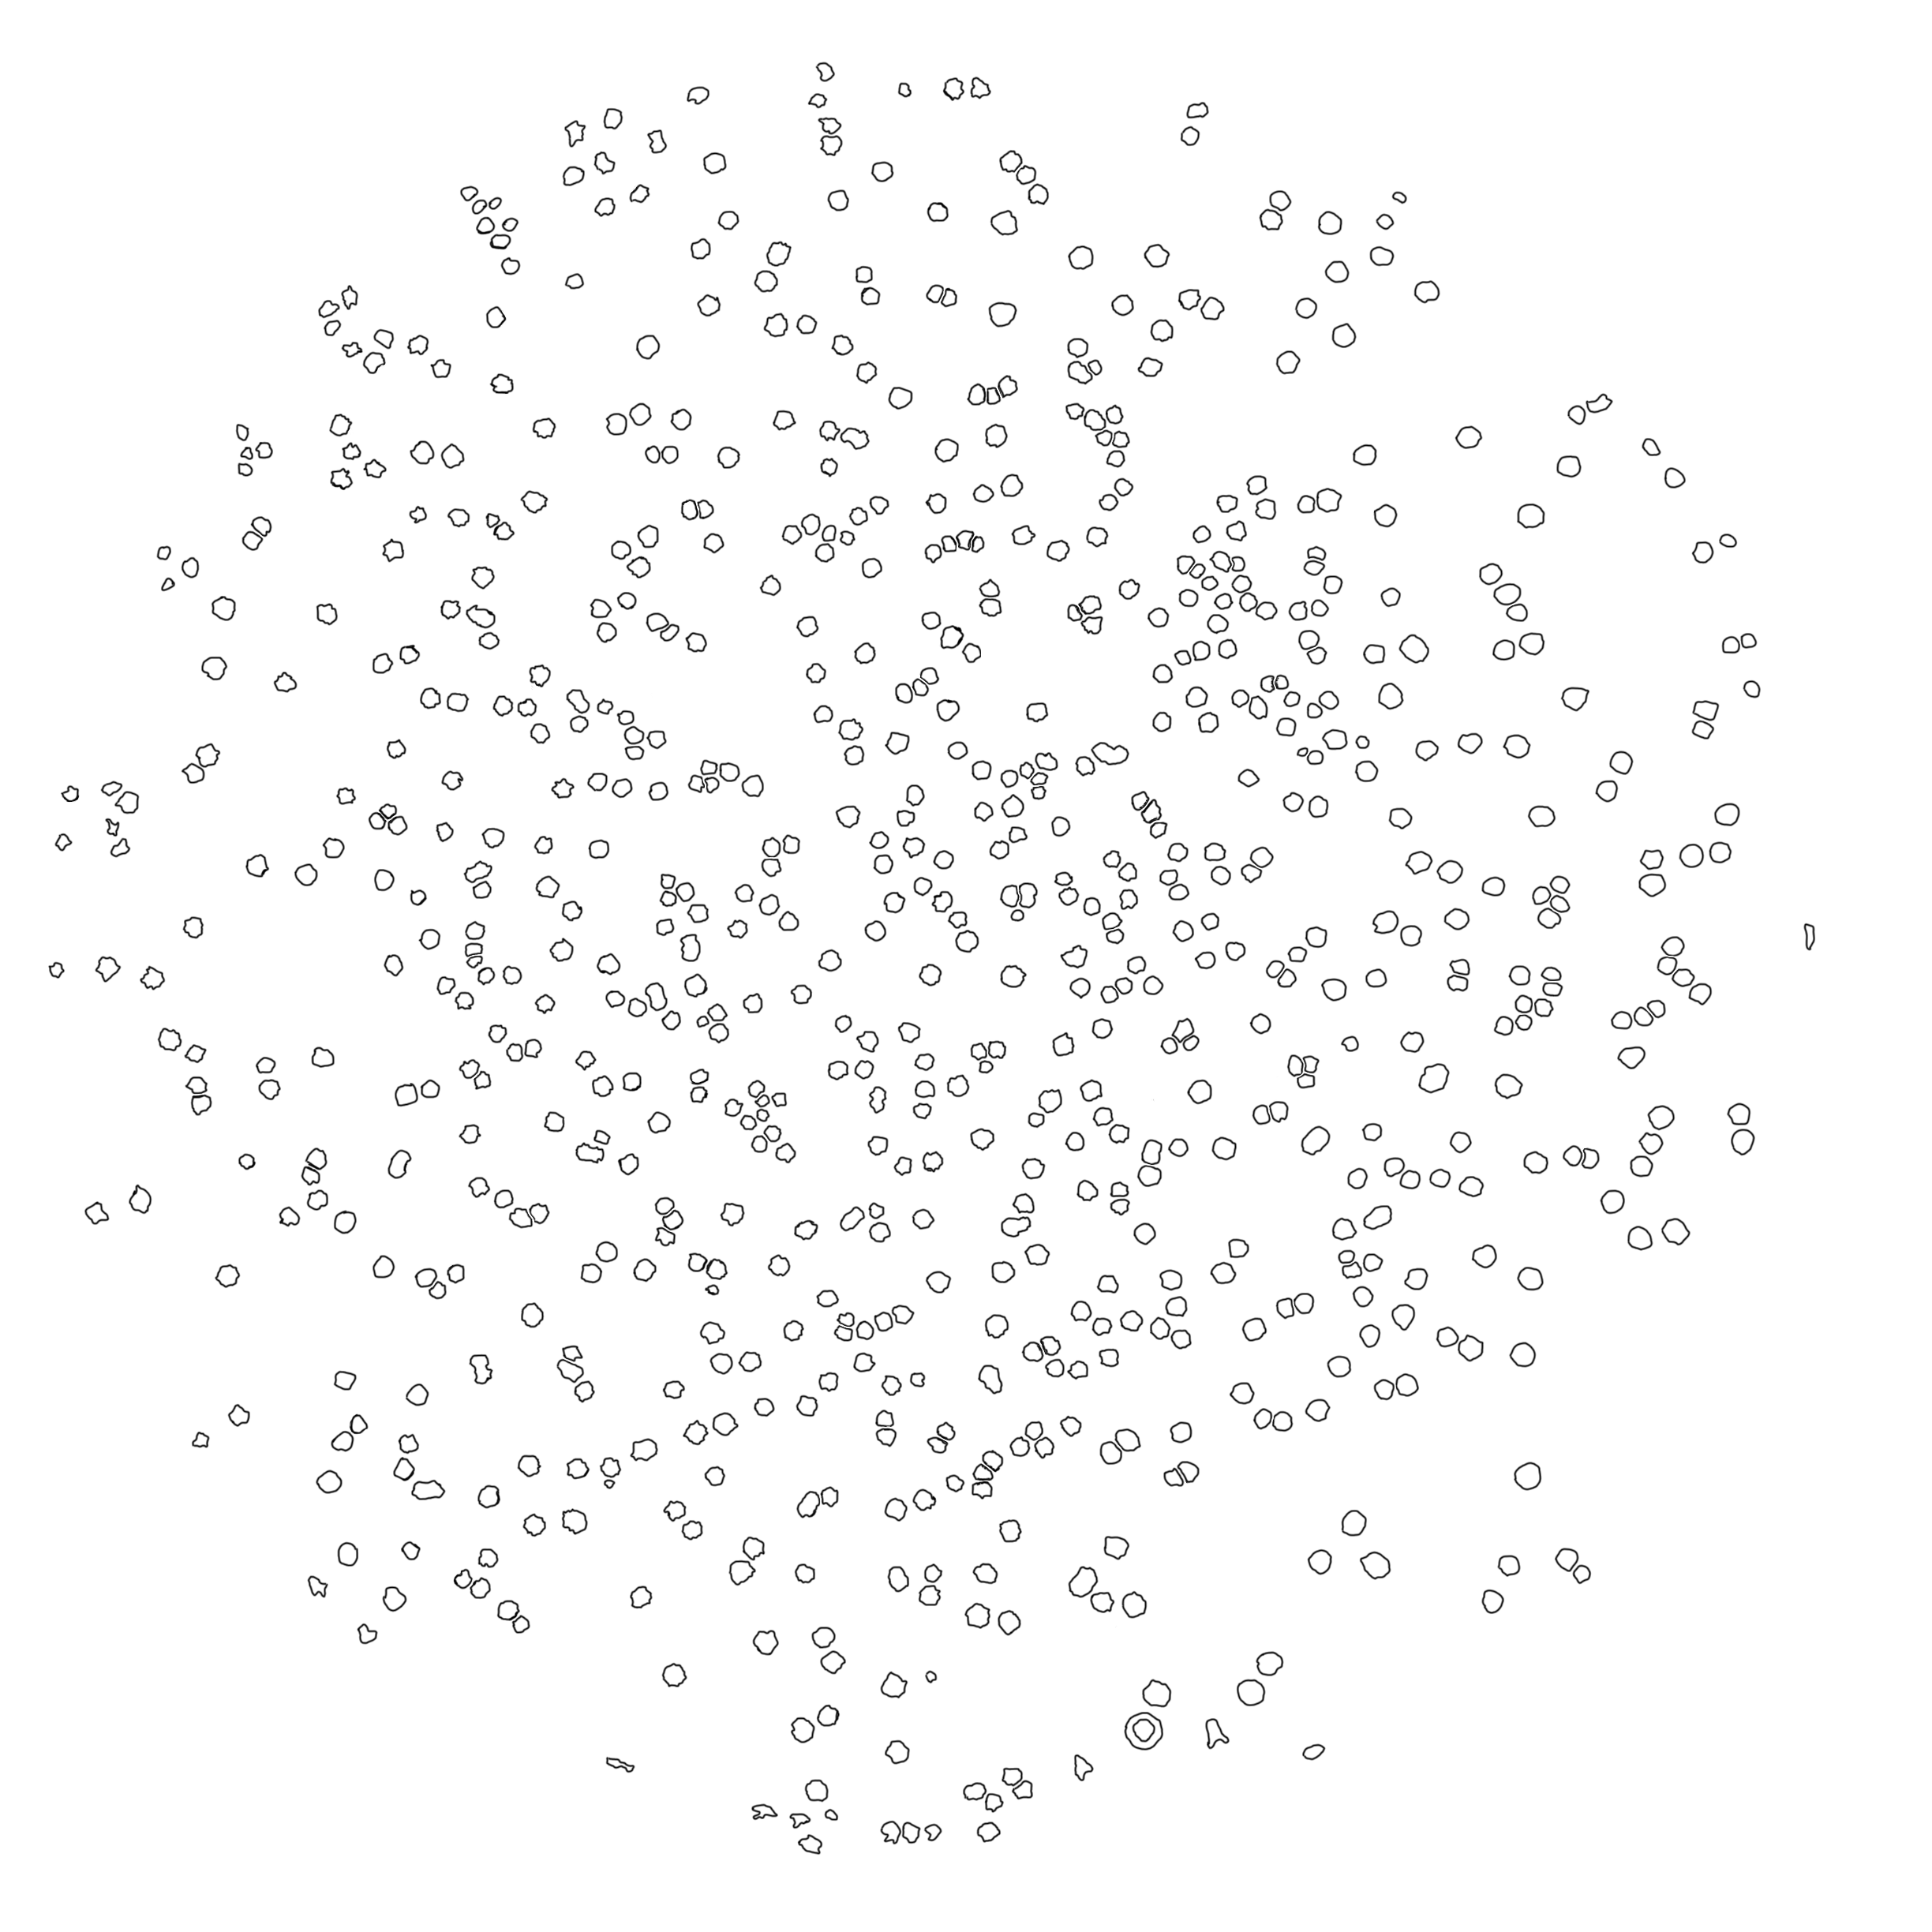
\includegraphics[width=0.2\textwidth]{easy_0_edge}
                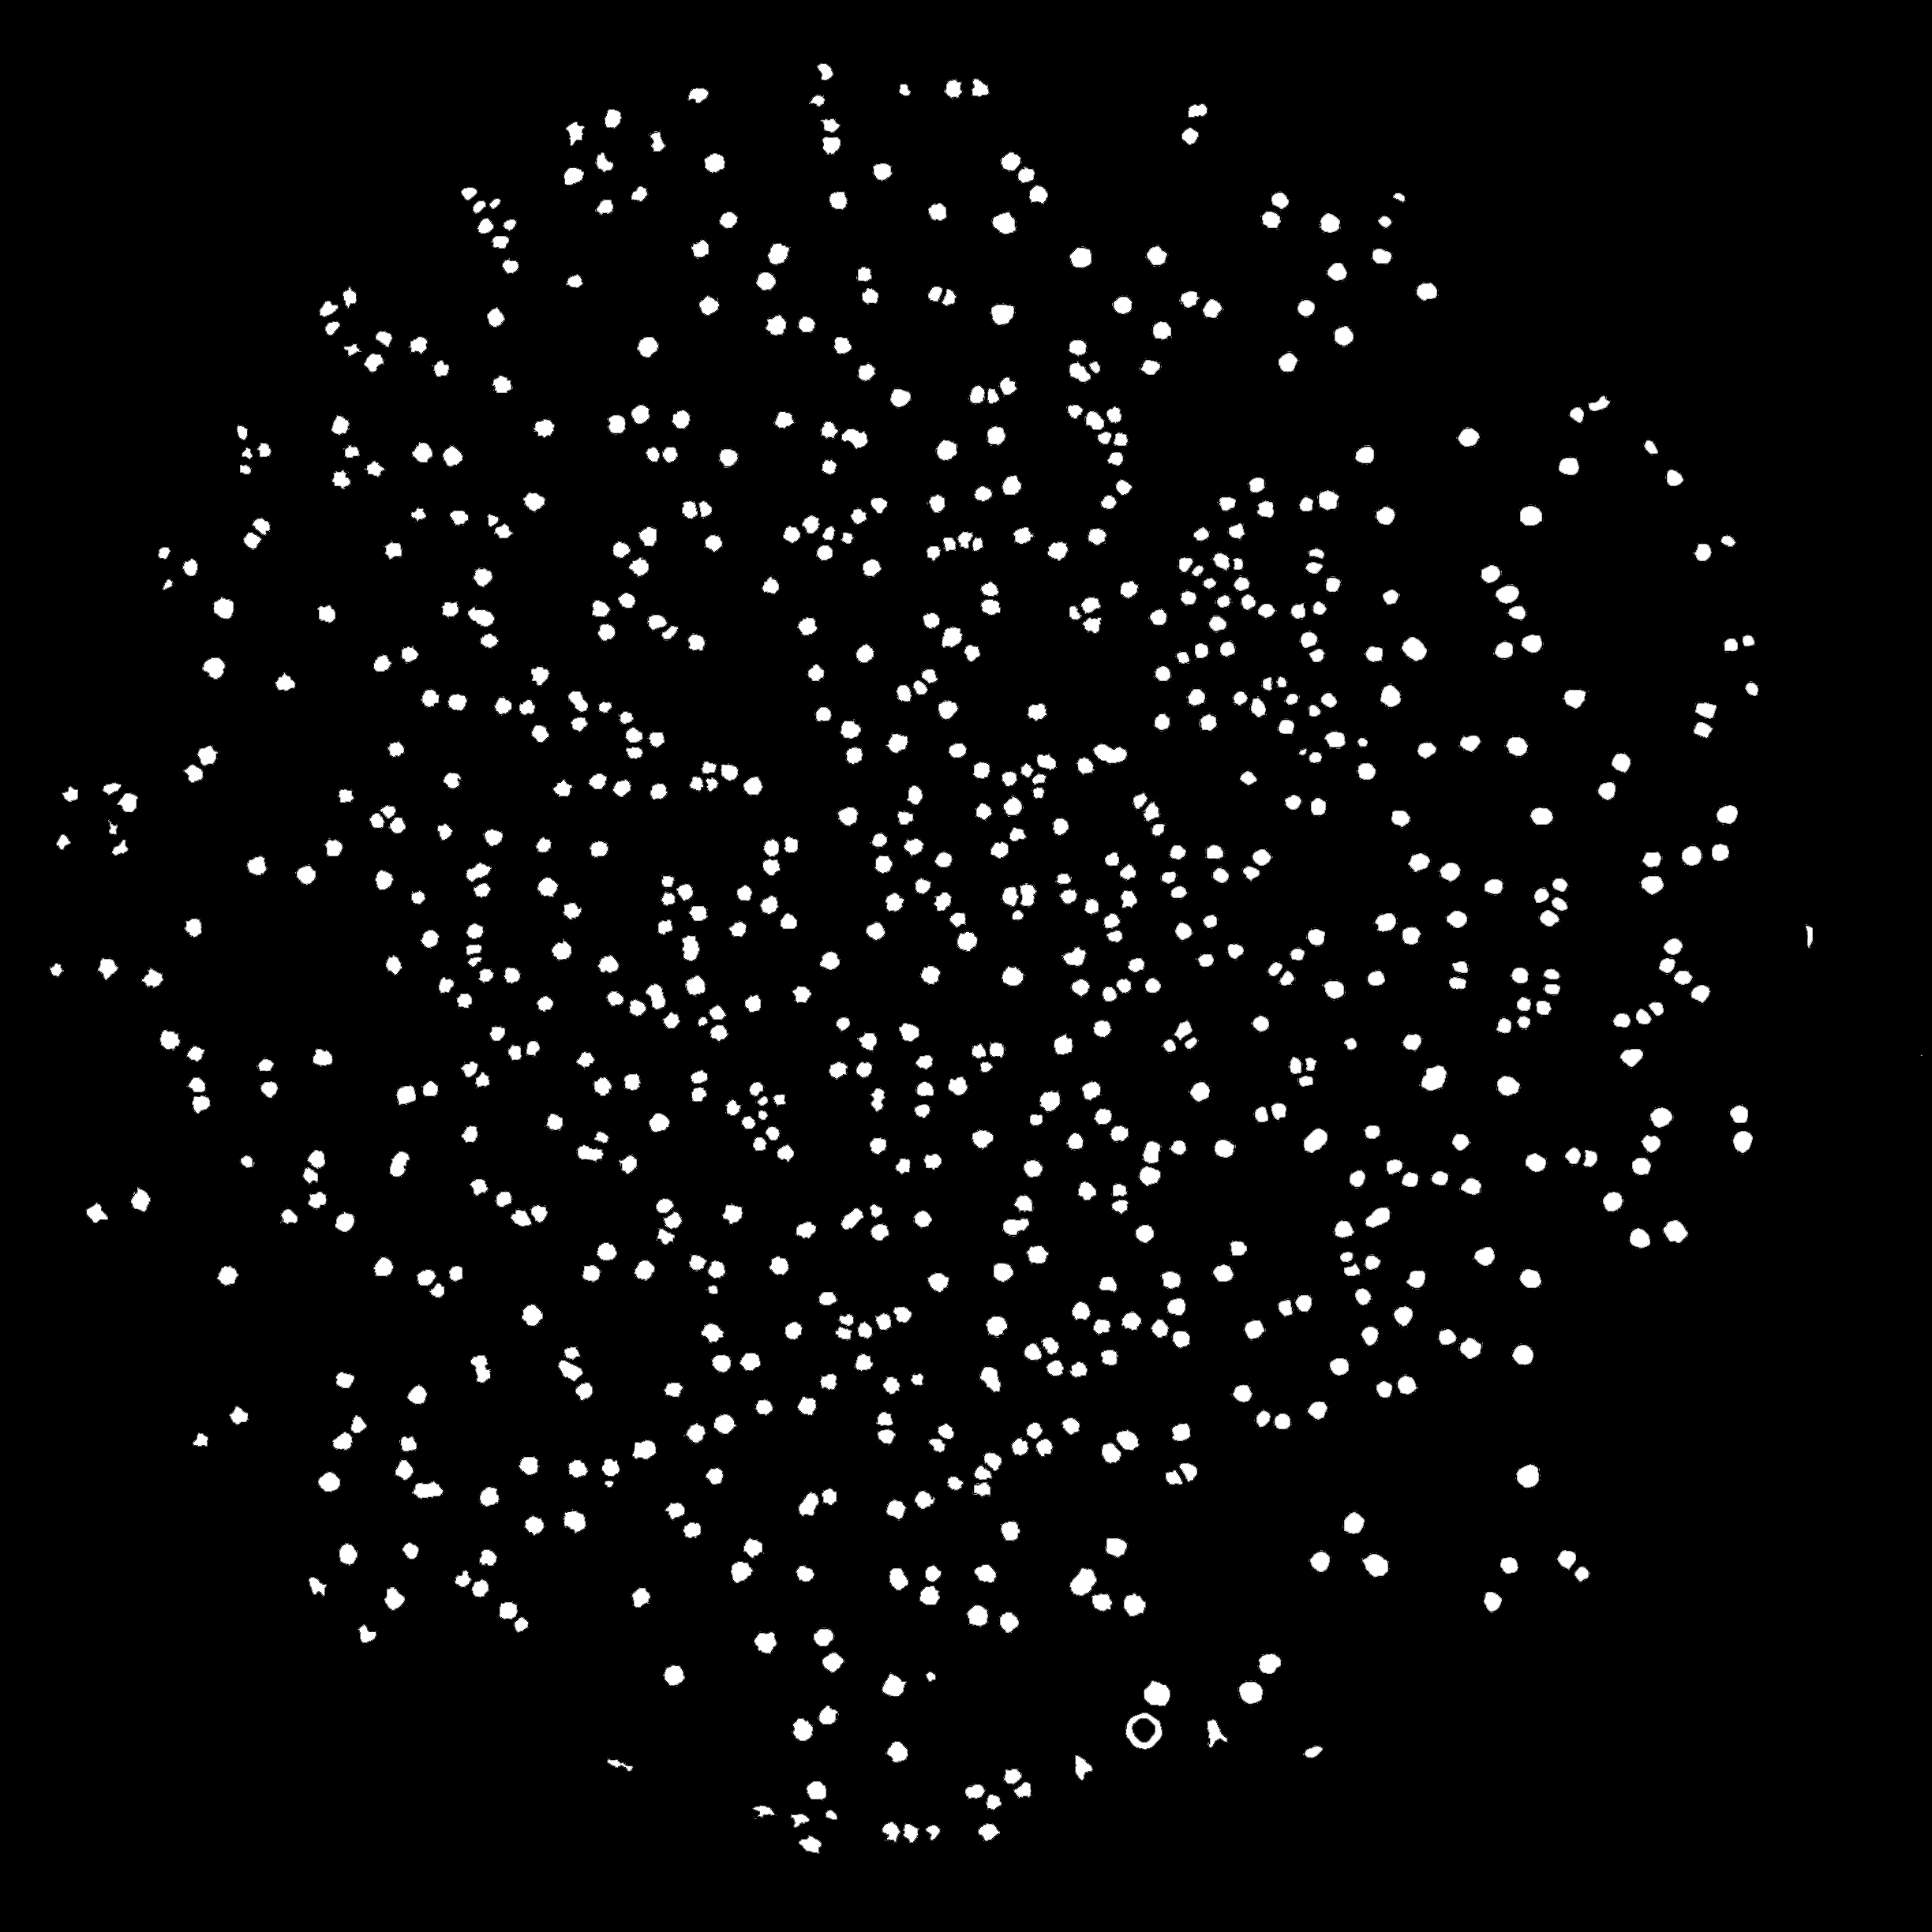
\includegraphics[width=0.2\textwidth]{easy_0_outside}
                \caption{{\bf Example of \texttt{easy\_masked} Dataset.} From left to right is the plate image, its \texttt{inside}-CFU mask, its \texttt{edge}-of-CFU mask, and its \texttt{outside}-all-CFUs mask.}
                \label{easy-masked}
            \end{figure}

        \paragraph*{\texttt{more\_masked} Dataset}
            This dataset contains the same components as $\texttt{easy\_masked}$. It has only $1$ plate, of a different bacterial strain, whose colonies have different size and morphology. It can be seen in Fig.~\ref{more-masked}. This dataset is used for training the DCNN.
        
            \begin{figure}[h]
                \graphicspath{{results/preprocess_masked/figures/original/}}
                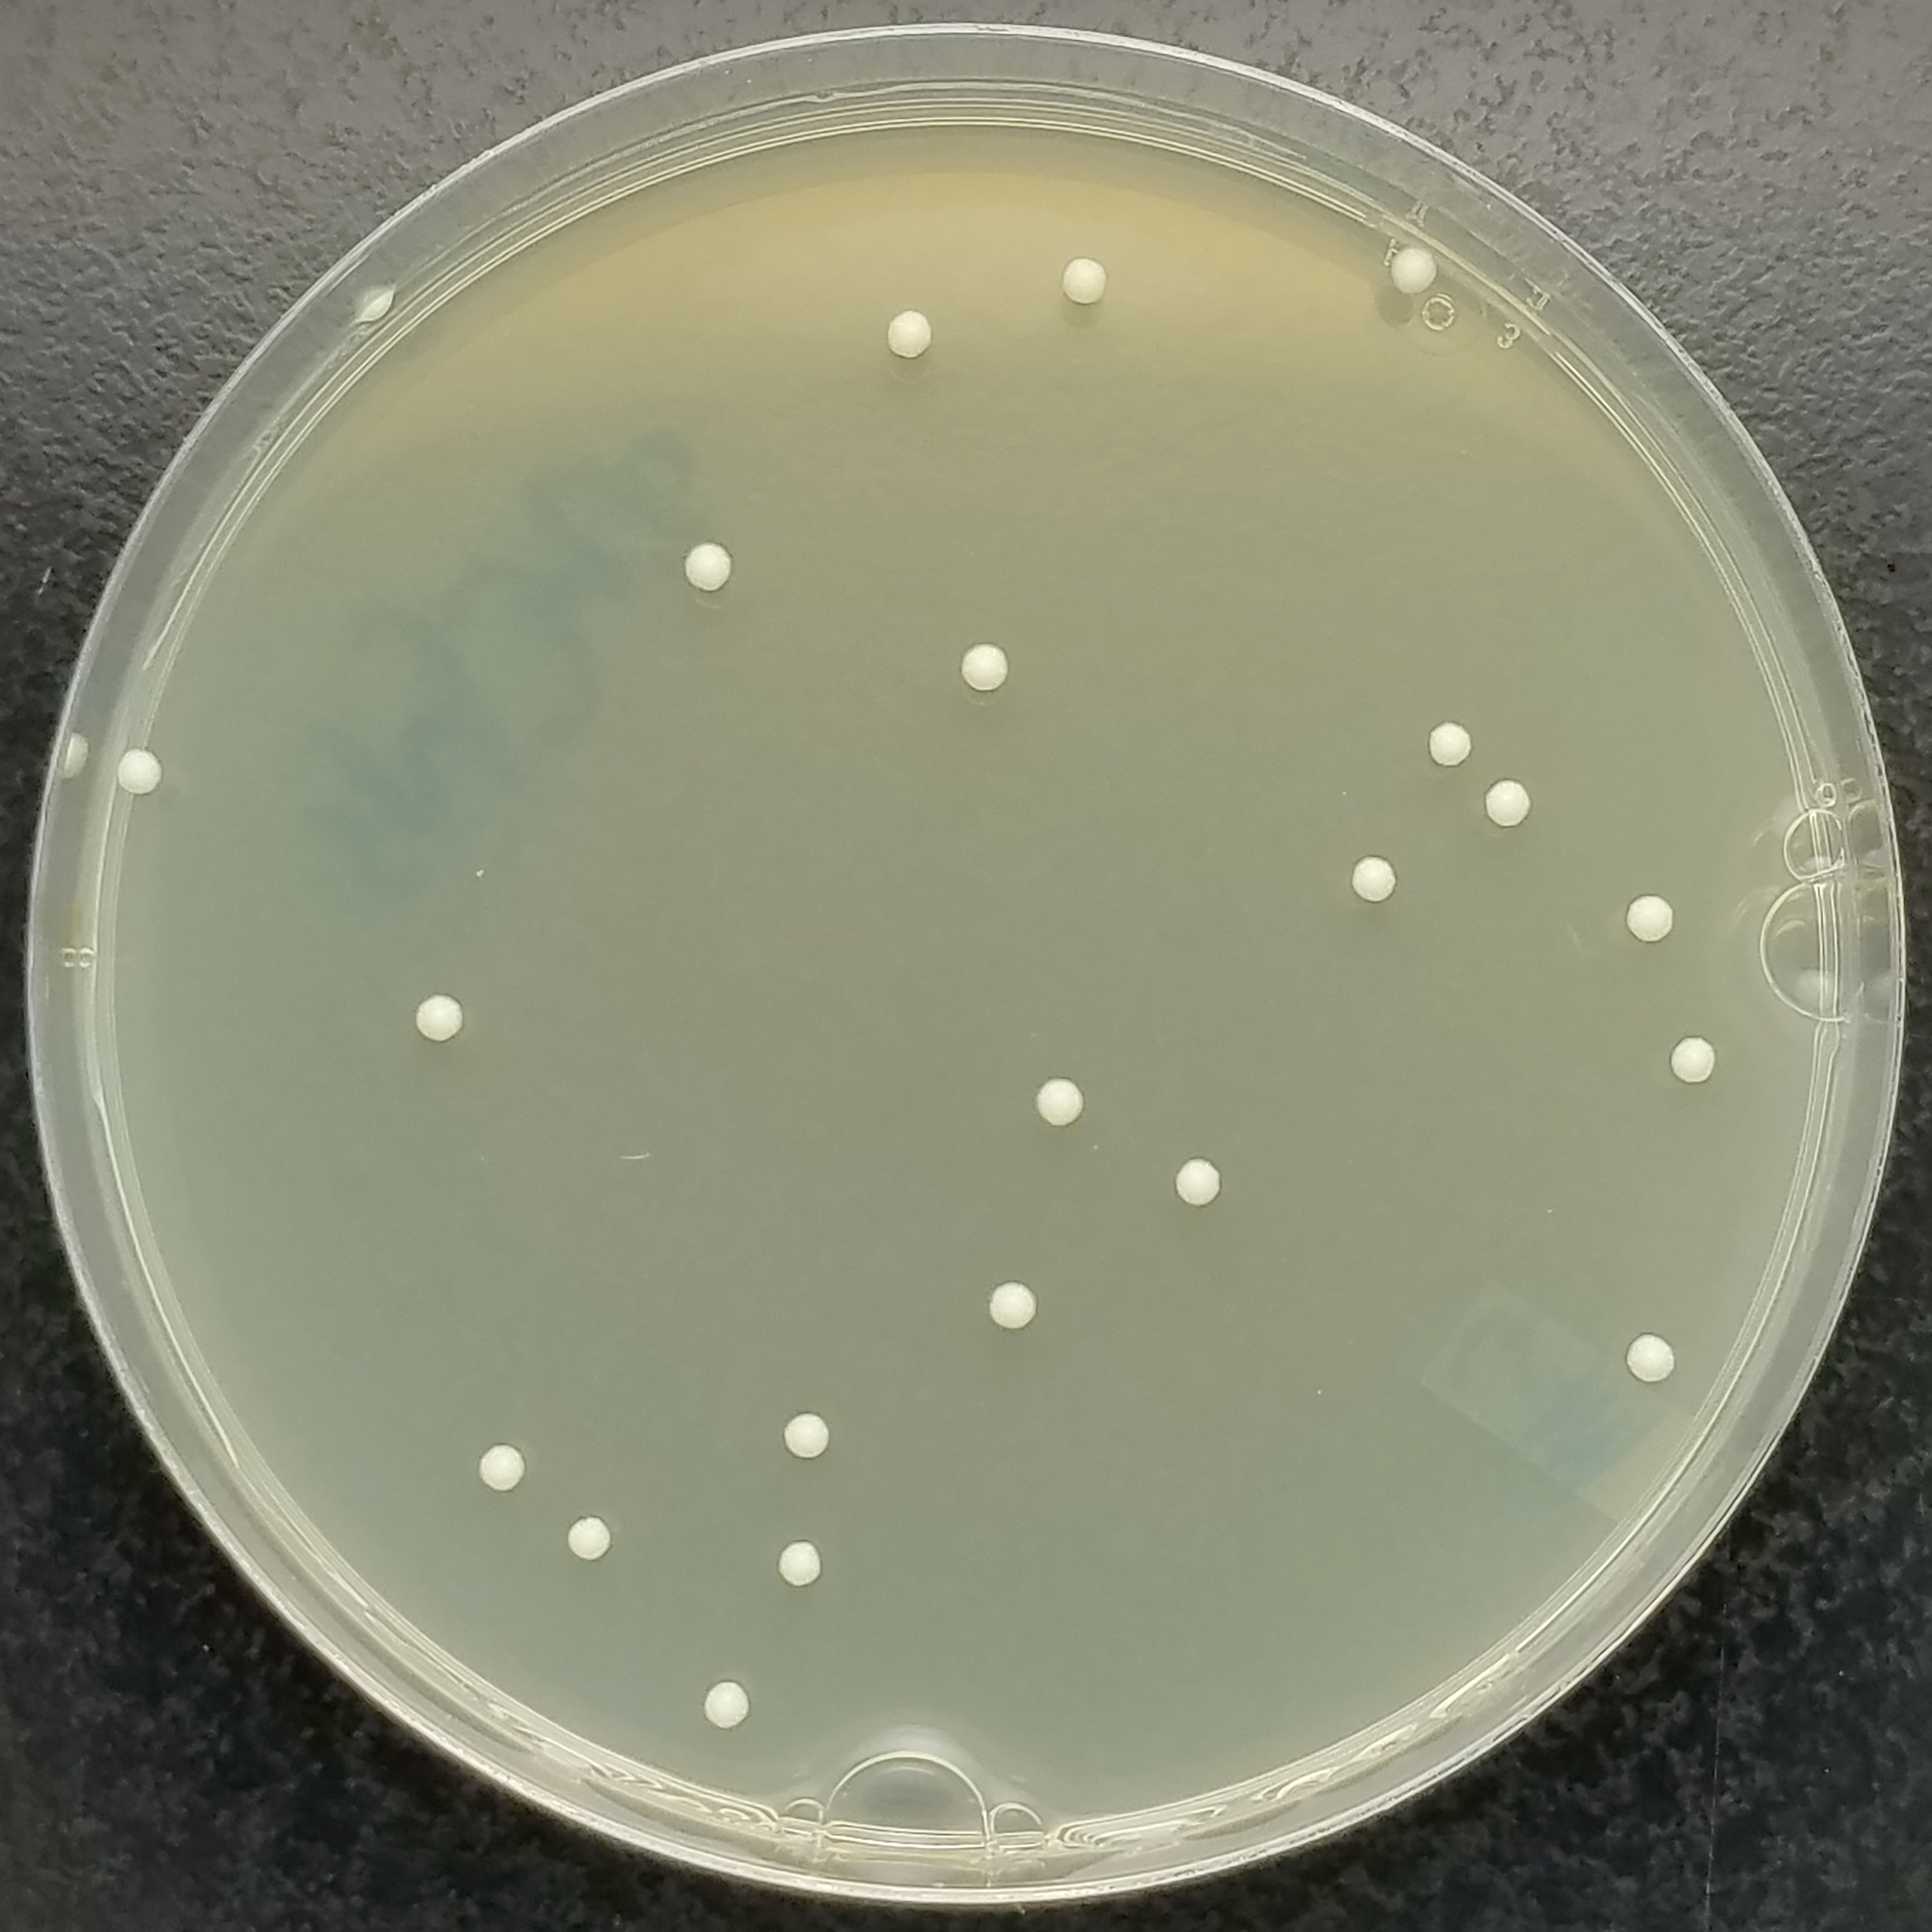
\includegraphics[width=0.2\textwidth]{more_0_image}
                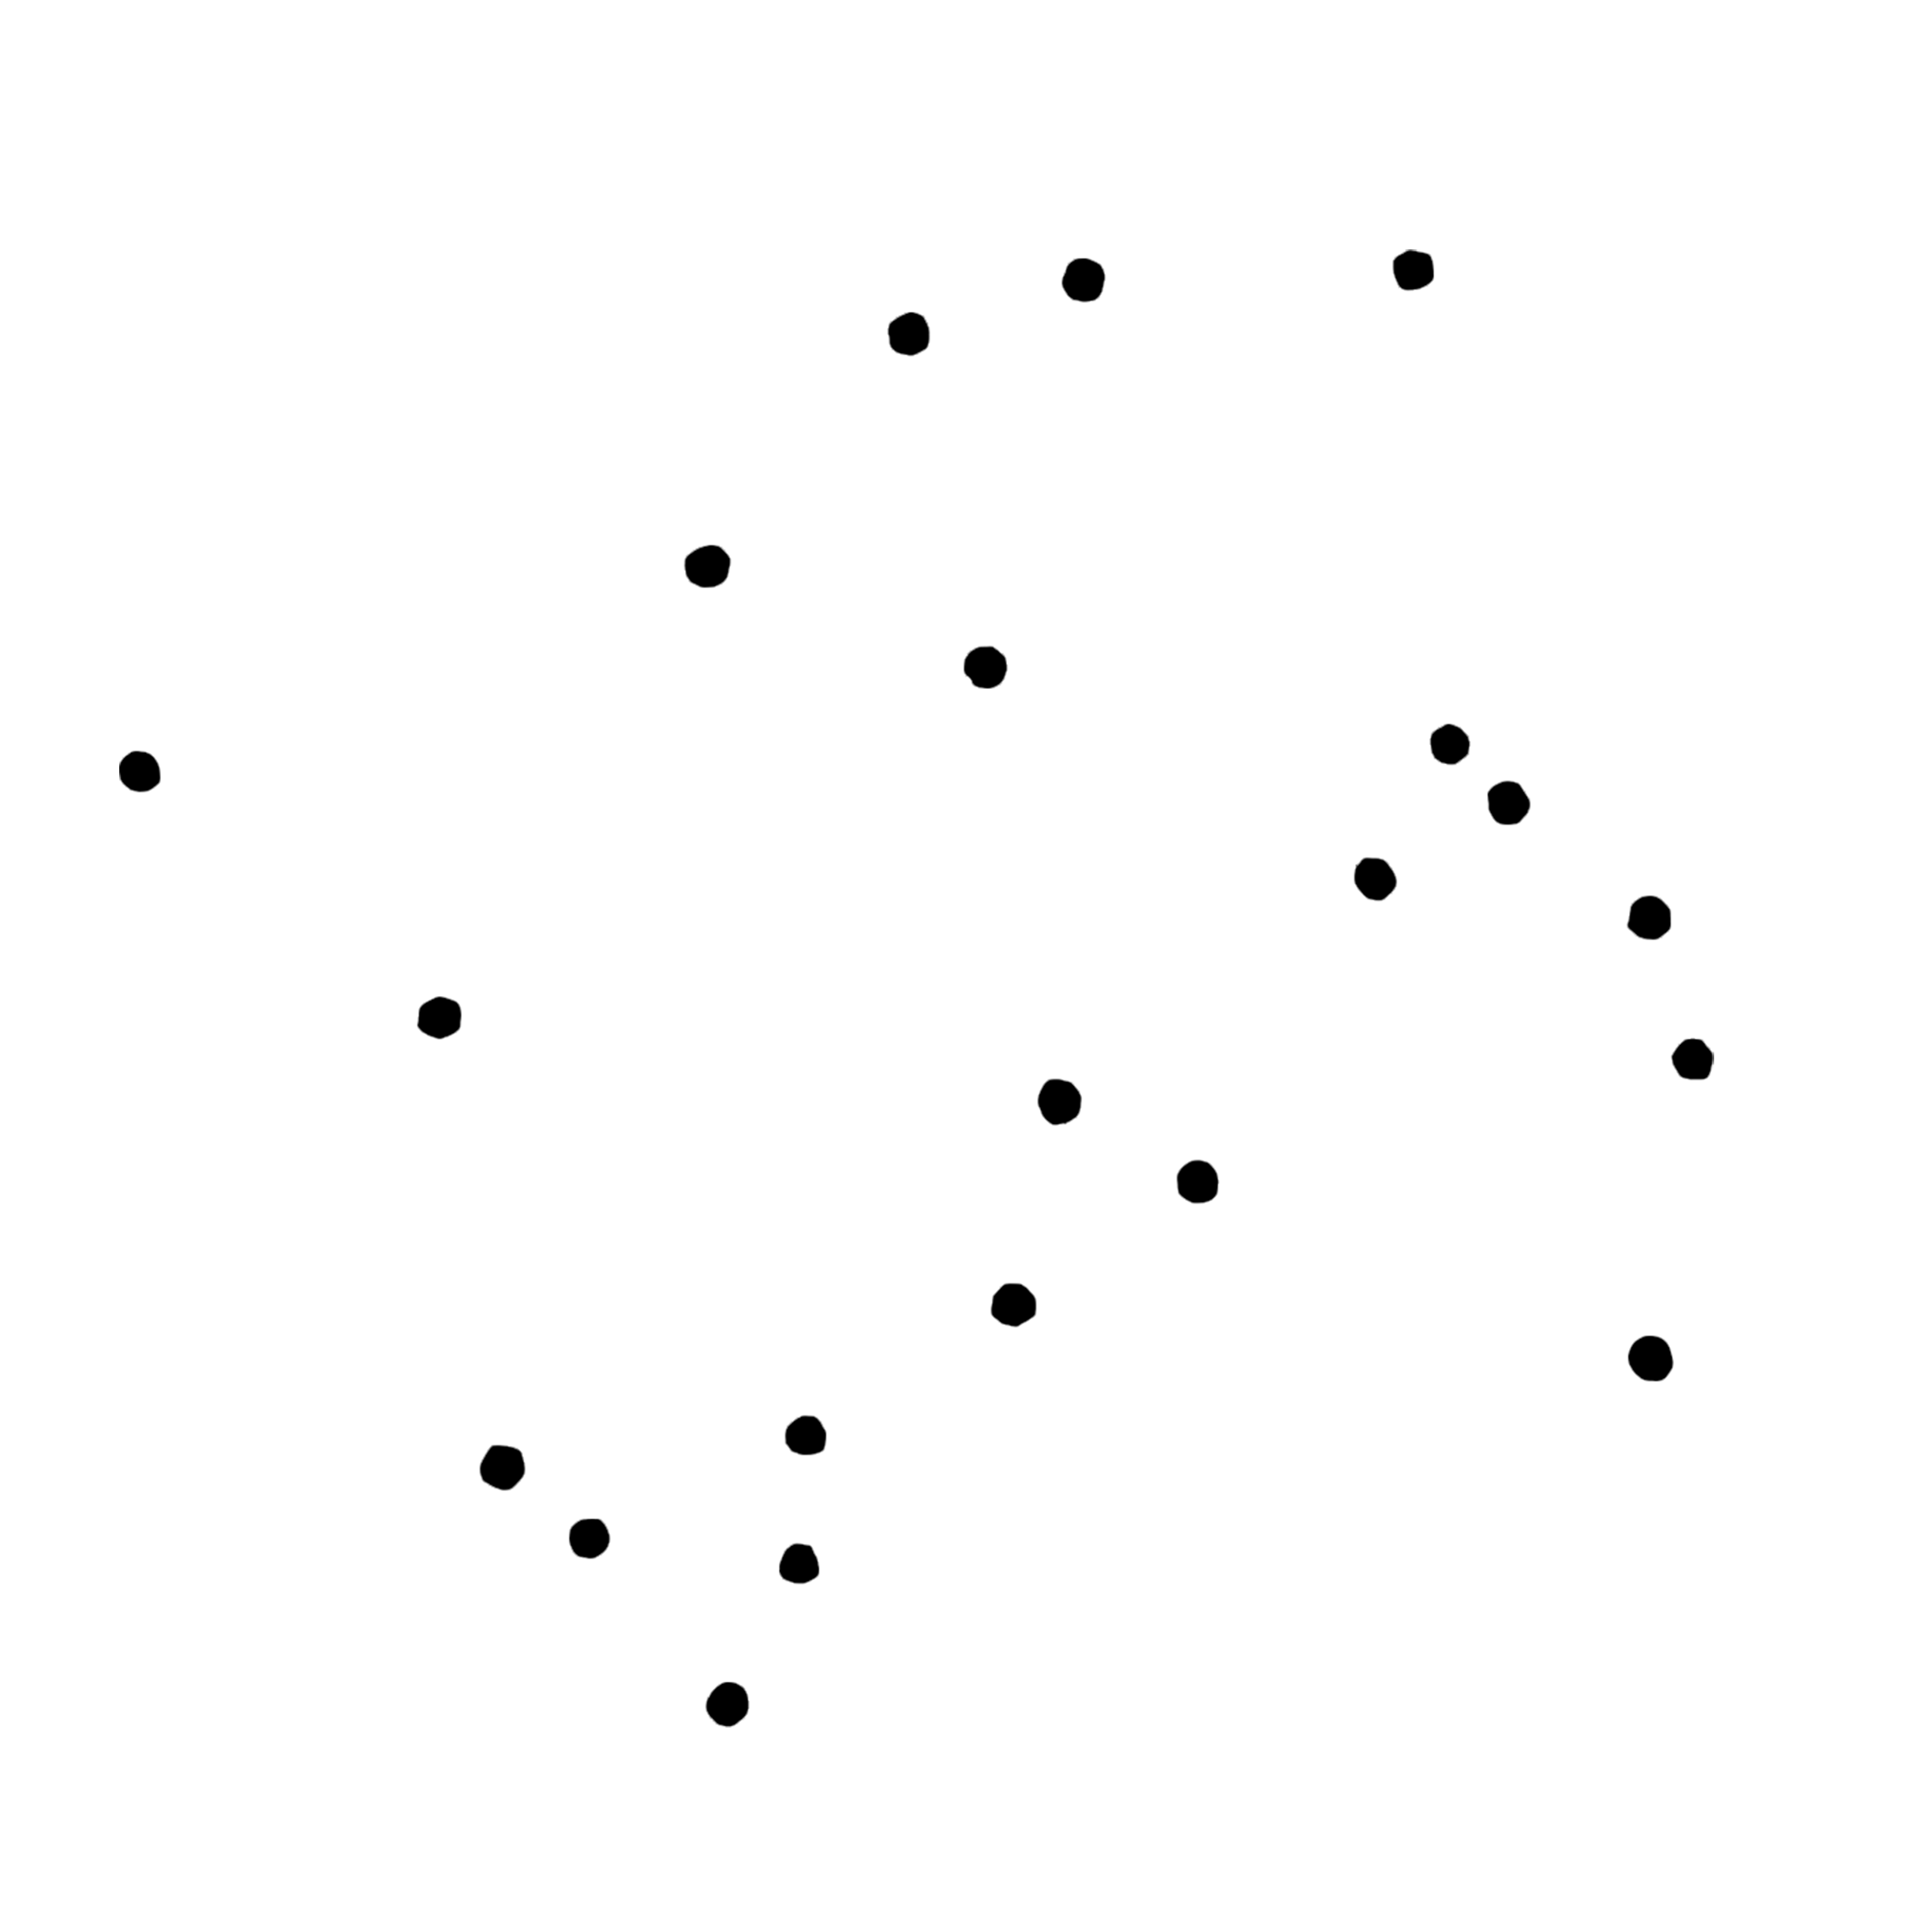
\includegraphics[width=0.2\textwidth]{more_0_inside}
                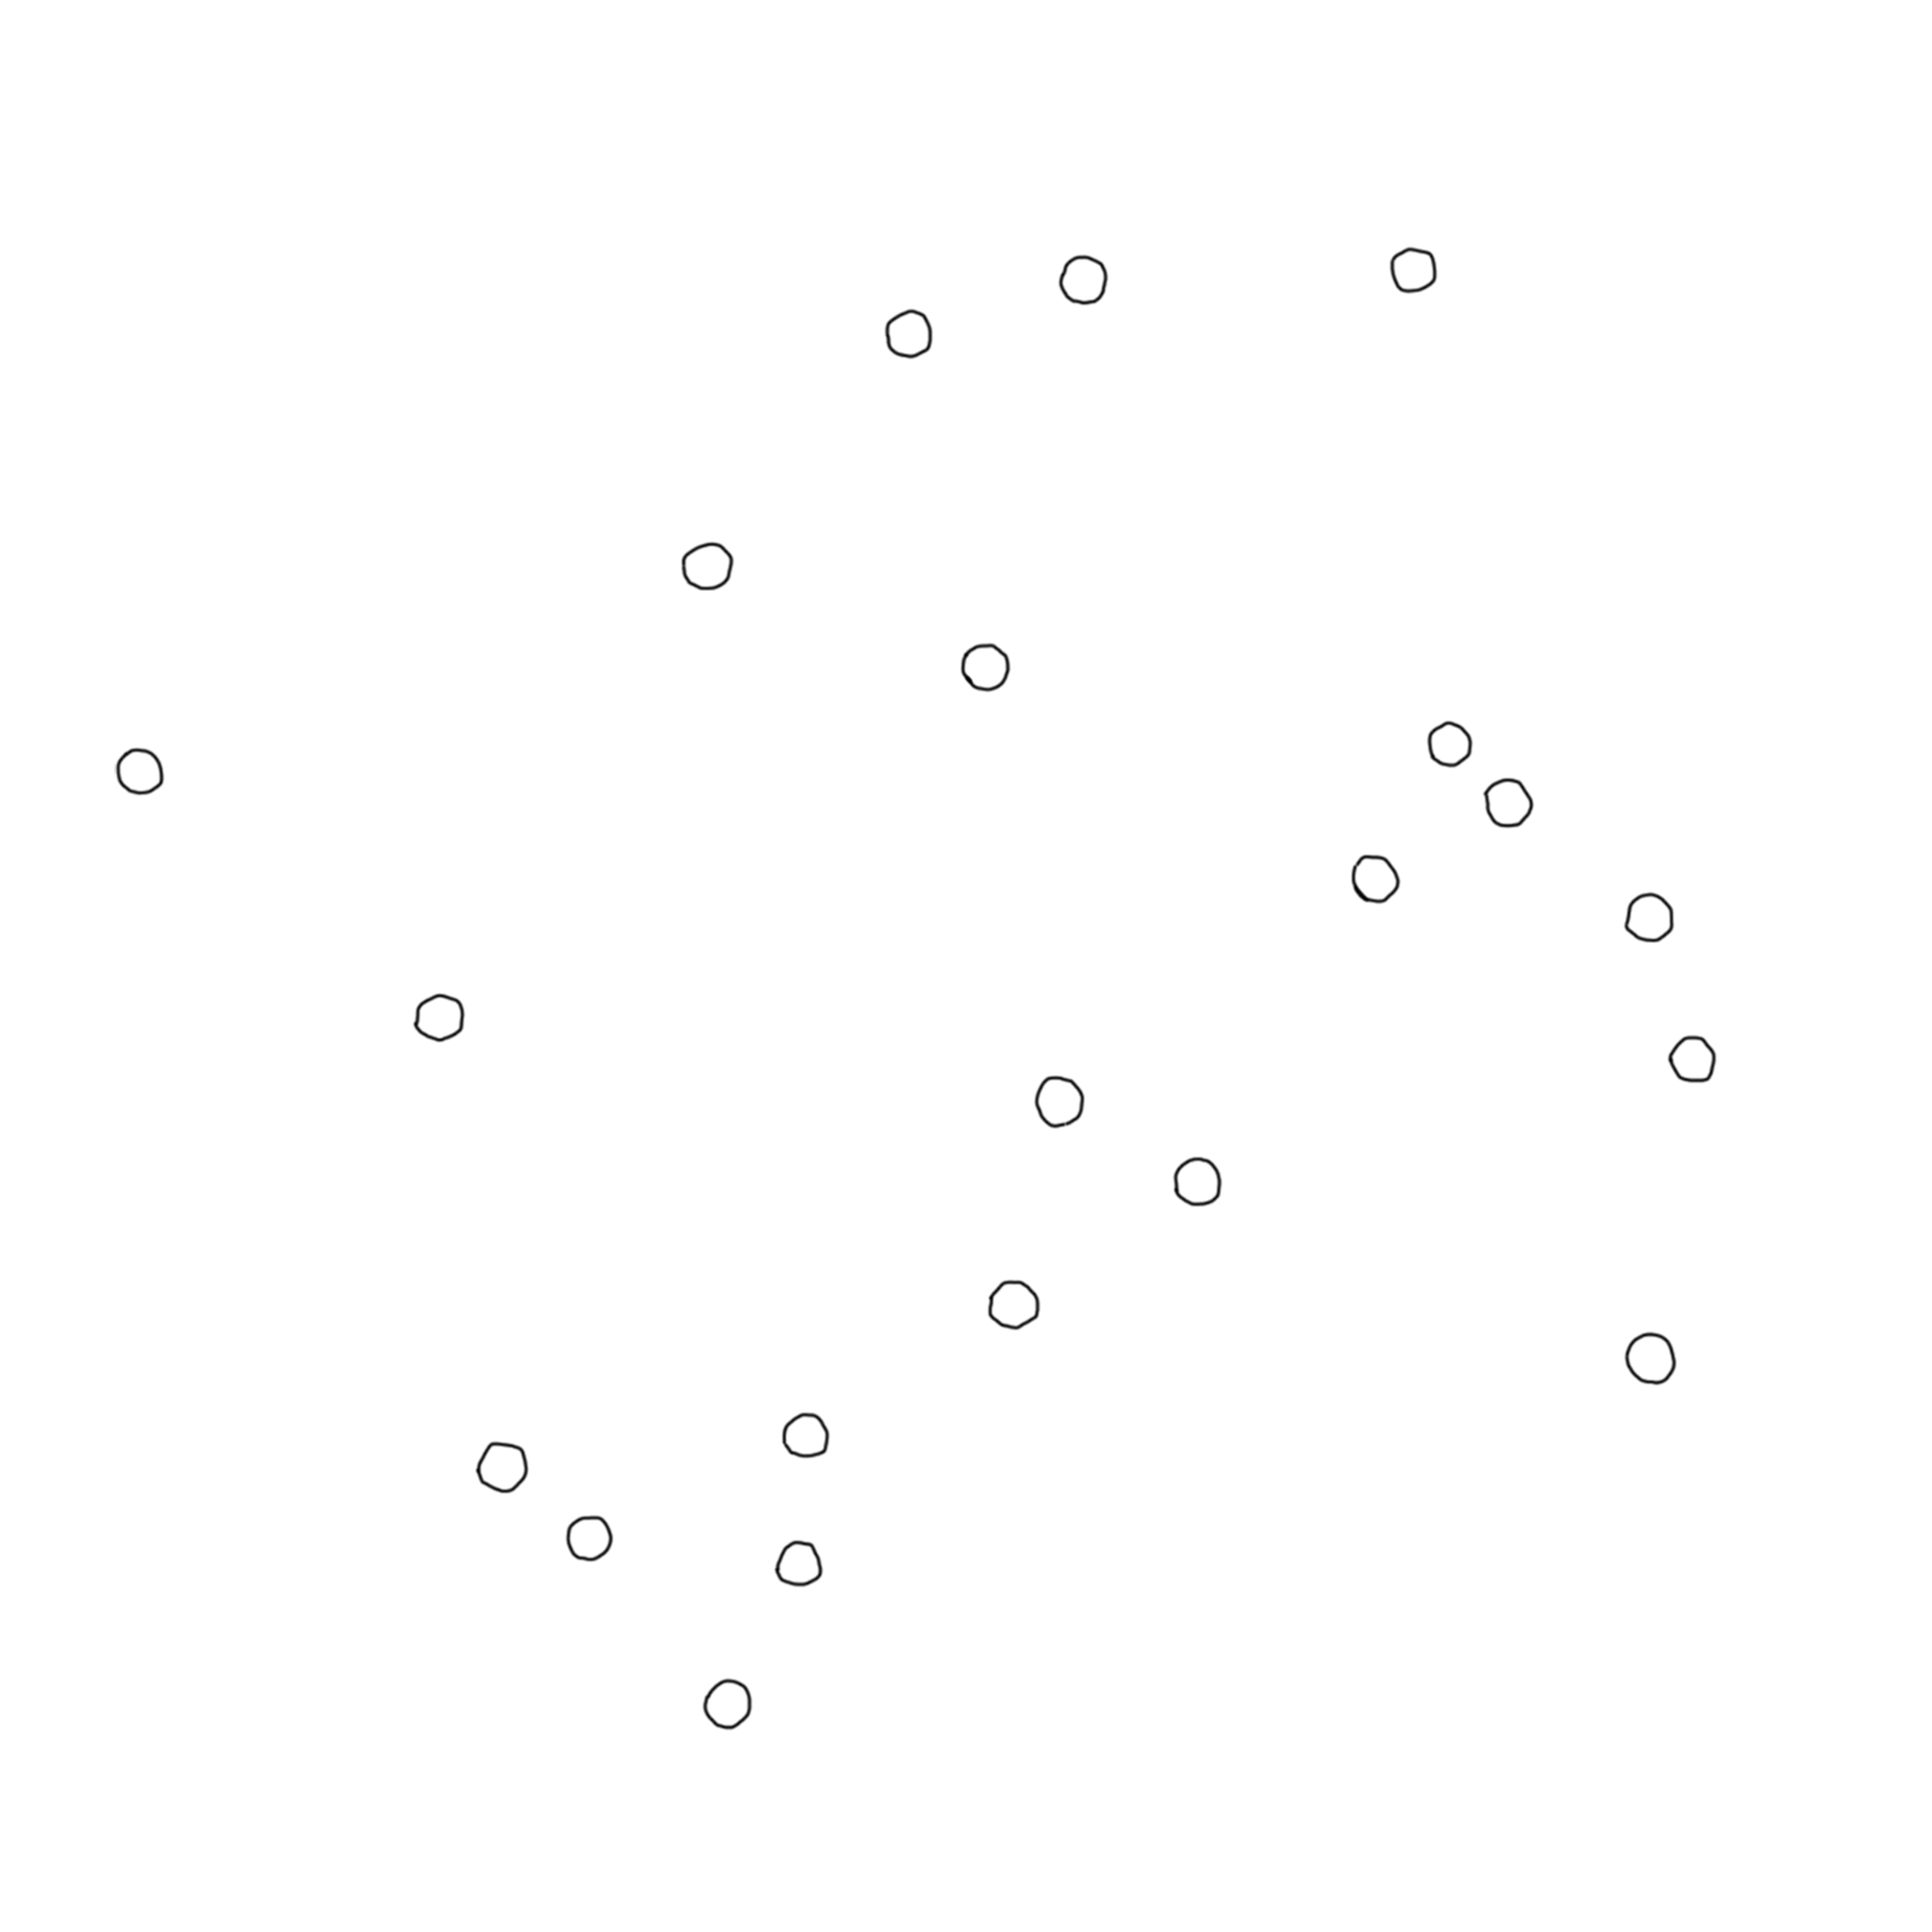
\includegraphics[width=0.2\textwidth]{more_0_edge}
                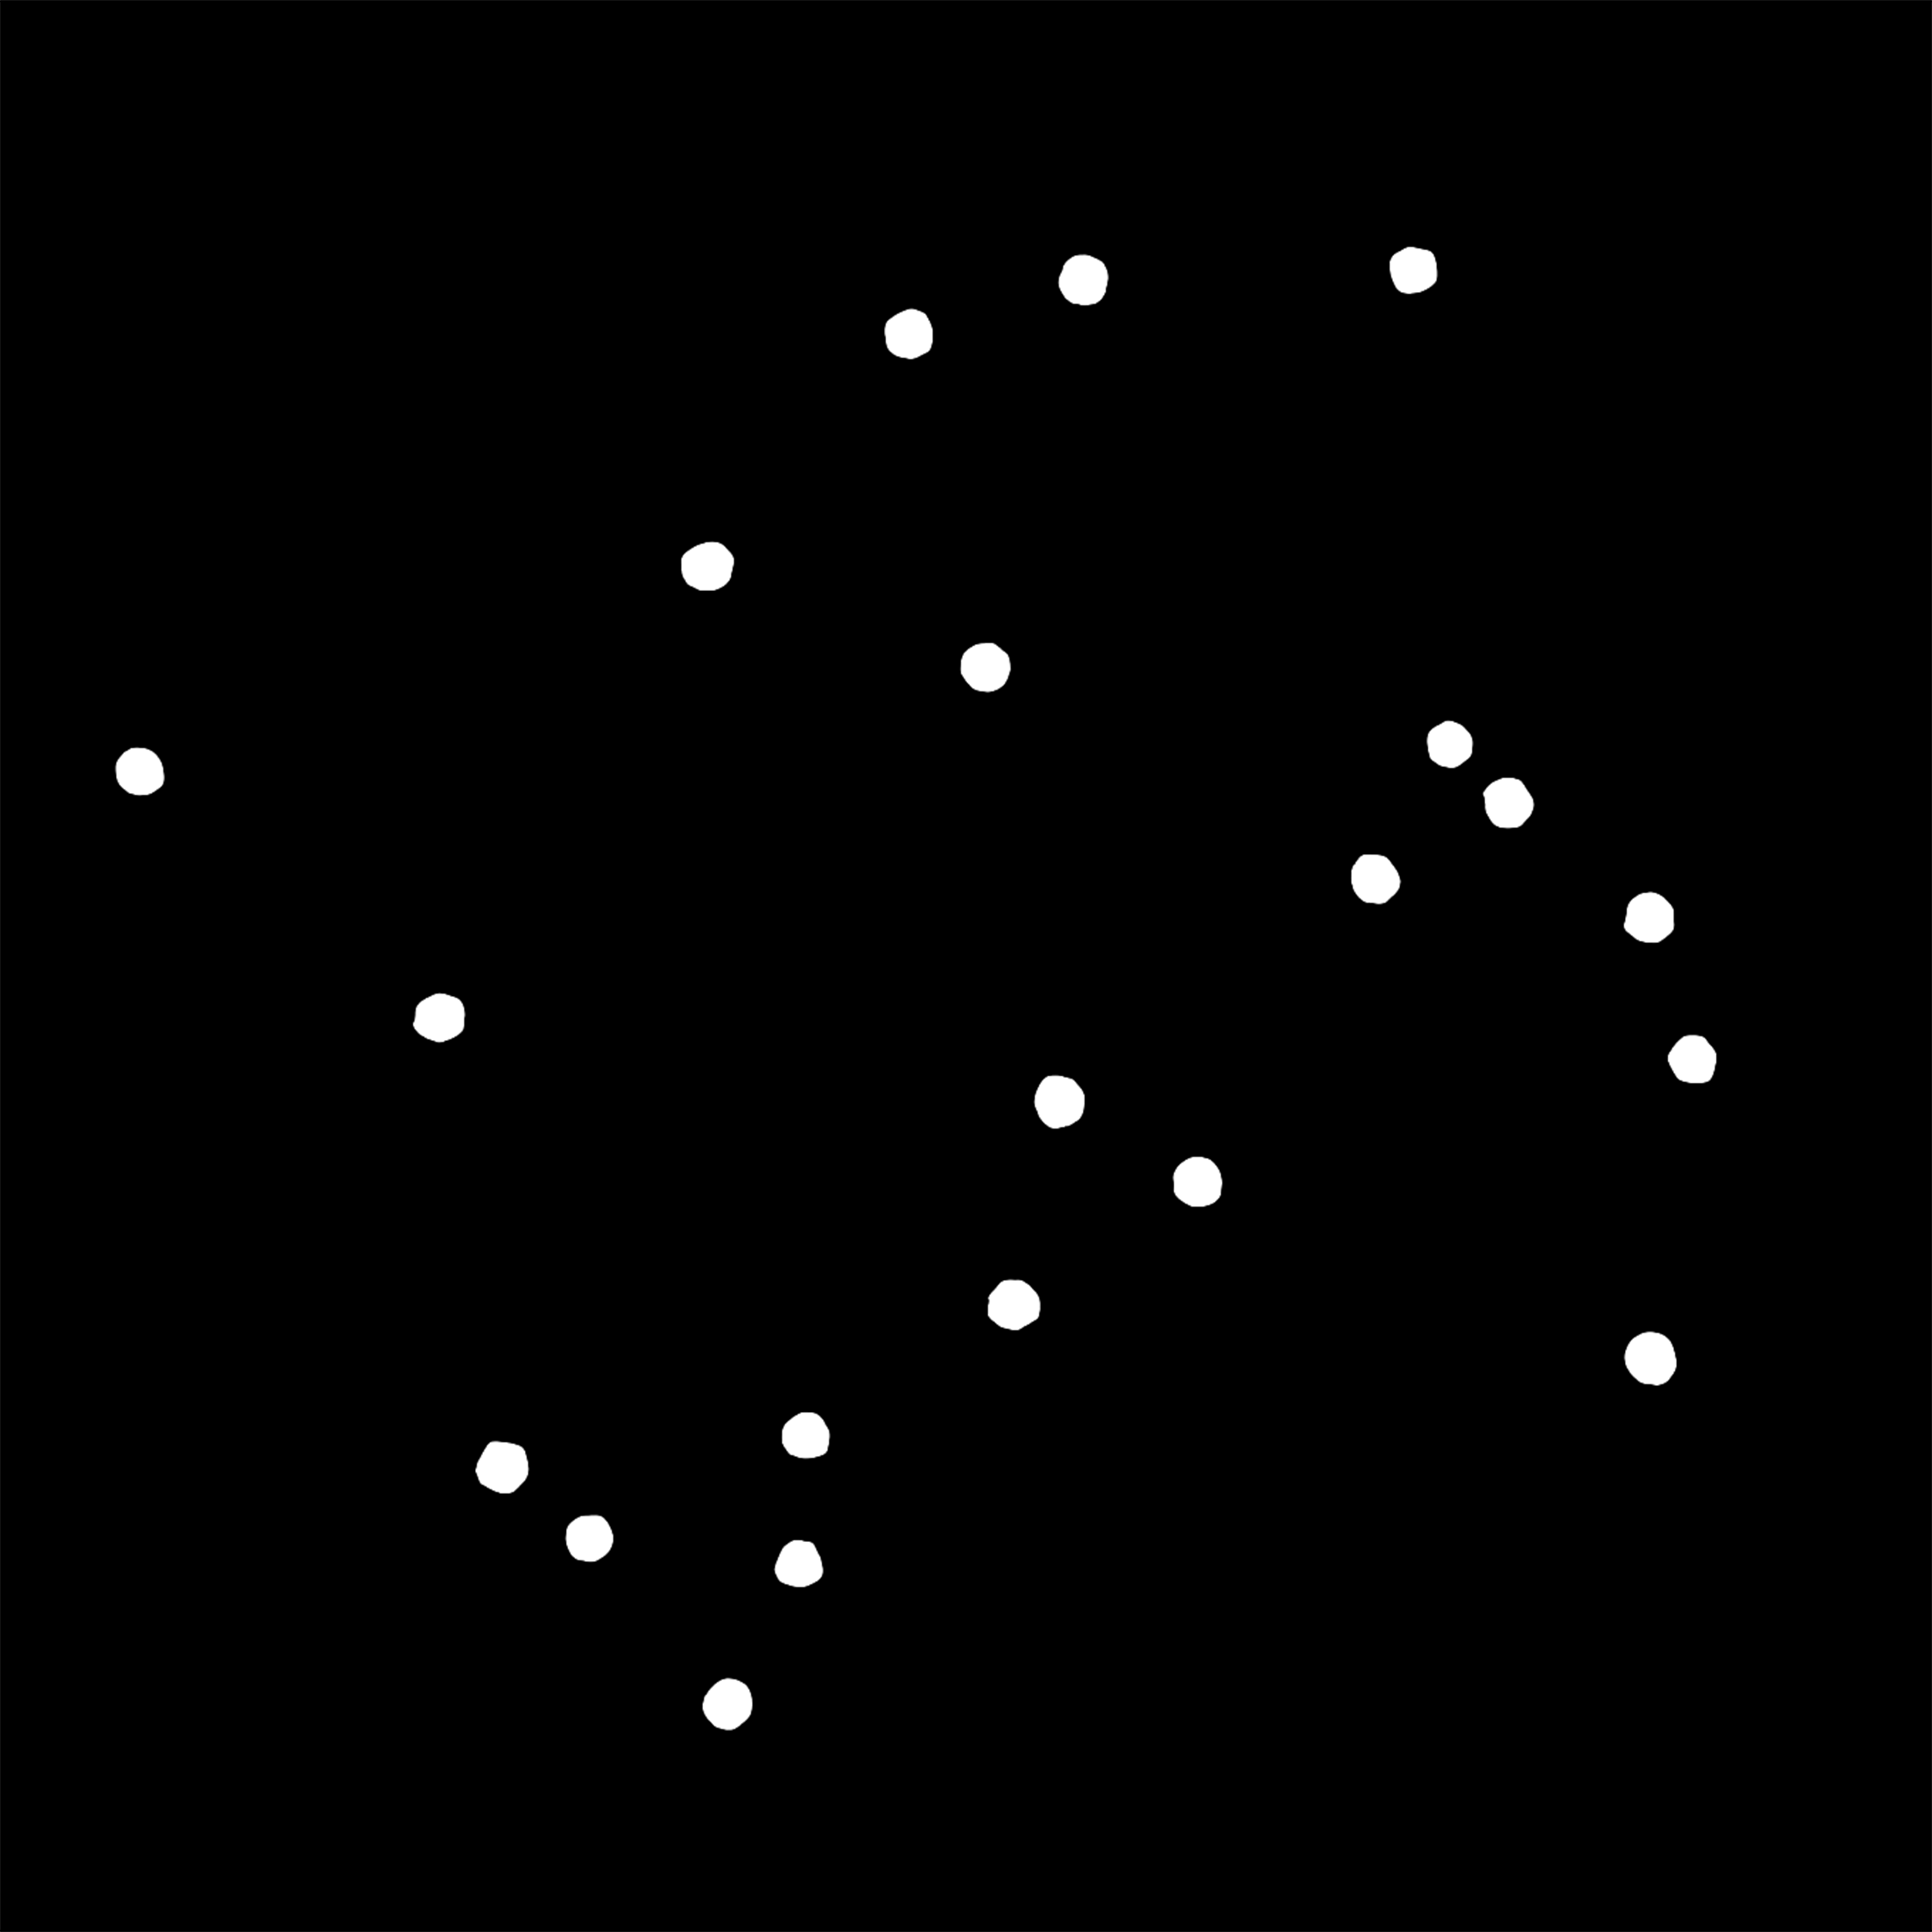
\includegraphics[width=0.2\textwidth]{more_0_outside}
                \caption{{\bf Example of \texttt{more\_masked} Dataset.}}
                \label{more-masked}
            \end{figure}

        \paragraph*{\texttt{easy} Dataset}
            This dataset consists of $26$ plate images and their counts. It comes from the same batch of plates (with the same bacterial strain) as $\texttt{easy\_masked}$. The only difference is no masks have been made for these. This dataset is used for testing the DCNN.
            
        \paragraph*{\texttt{more} Dataset}
            This dataset consists of $2$ plate images and their counts. It comes from the same batch of plates (with the same bacterial strain) as $\texttt{more}$. The only difference is no masks have been made for these. This dataset is used for testing the DCNN.

        \paragraph*{\texttt{multi} Dataset}
            This dataset consists of $3$ plates images, each photographed under $3$ conditions, as well as the plates' counts. The conditions are listed below. It can be seen in Fig.~\ref{multi}. This dataset is used for testing the DCNN.

            \begin{enumerate}
                \item $\texttt{light\_uncovered\_far\_noperspective}$: Photographed with extra lighting, with the plate's cover removed, from about $1ft$ away, with no perspective
                \item $\texttt{nolight\_uncovered\_close\_minorperspective}$: Photographed without extra lighting, with the plate's cover removed, from about $3in$ away, with minor perspective
                \item $\texttt{light\_covered\_close\_severeperspective}$: Photographed with extra lighting, with the plate's cover on, from about $3in$ away, with severe perspective.
            \end{enumerate}
            
            \begin{figure}[h]
                \includesvg[svgpath=results/preprocess_multi/figures/, width=0.7\textwidth]{plate_0}
                \caption{{\bf Example of \texttt{multi} Dataset.}}
                \label{multi}
            \end{figure}

        \paragraph*{\texttt{pinned} Dataset}    
            This dataset consists of $417$ well images and their counts. The well images are extracted from a set of $32$ images of 96-well plates. It can be seen in Fig.~\ref{pinned}. This dataset is used for testing the DCNN, as well as training, validating, and testing the SVM.
            
            \begin{figure}[h]
                \includesvg[svgpath=results/preprocess_pinned/figures/, width=0.7\textwidth]{plates_resized}
                \caption{{\bf Sample of \texttt{pinned} Dataset.}}
                \label{pinned}
            \end{figure}

    \subsection*{DCNN} \label{ssec:dcnn}
        \paragraph*{Summary}
            Our first model is a deep convolutional neural network (DCNN) that copies the architecture of \cite{Valen}. In brief, the model takes as input a $61px \times 61px$ image. It outputs a "class", one of \texttt{inside}, \texttt{edge}, or \texttt{outside}. Our goal is to be able to input a $61px \times 61px$ patch of a plate image and have the DCNN output whether the center pixel of the patch is \texttt{inside} a CFU, on the \texttt{edge} of some CFU(s), or \texttt{outside} all CFUs. We will then collect the \texttt{inside} classifications into an \texttt{inside}-a-CFU mask of the image, which constitutes a segmentation of the image. Then, we will use standard algorithms to clean up noise and count the number of segments present. This pipeline is depicted in Fig.~\cite{dcnn_pipeline}.
            
            \begin{figure}[h]
                \graphicspath{{results/derived/}}
                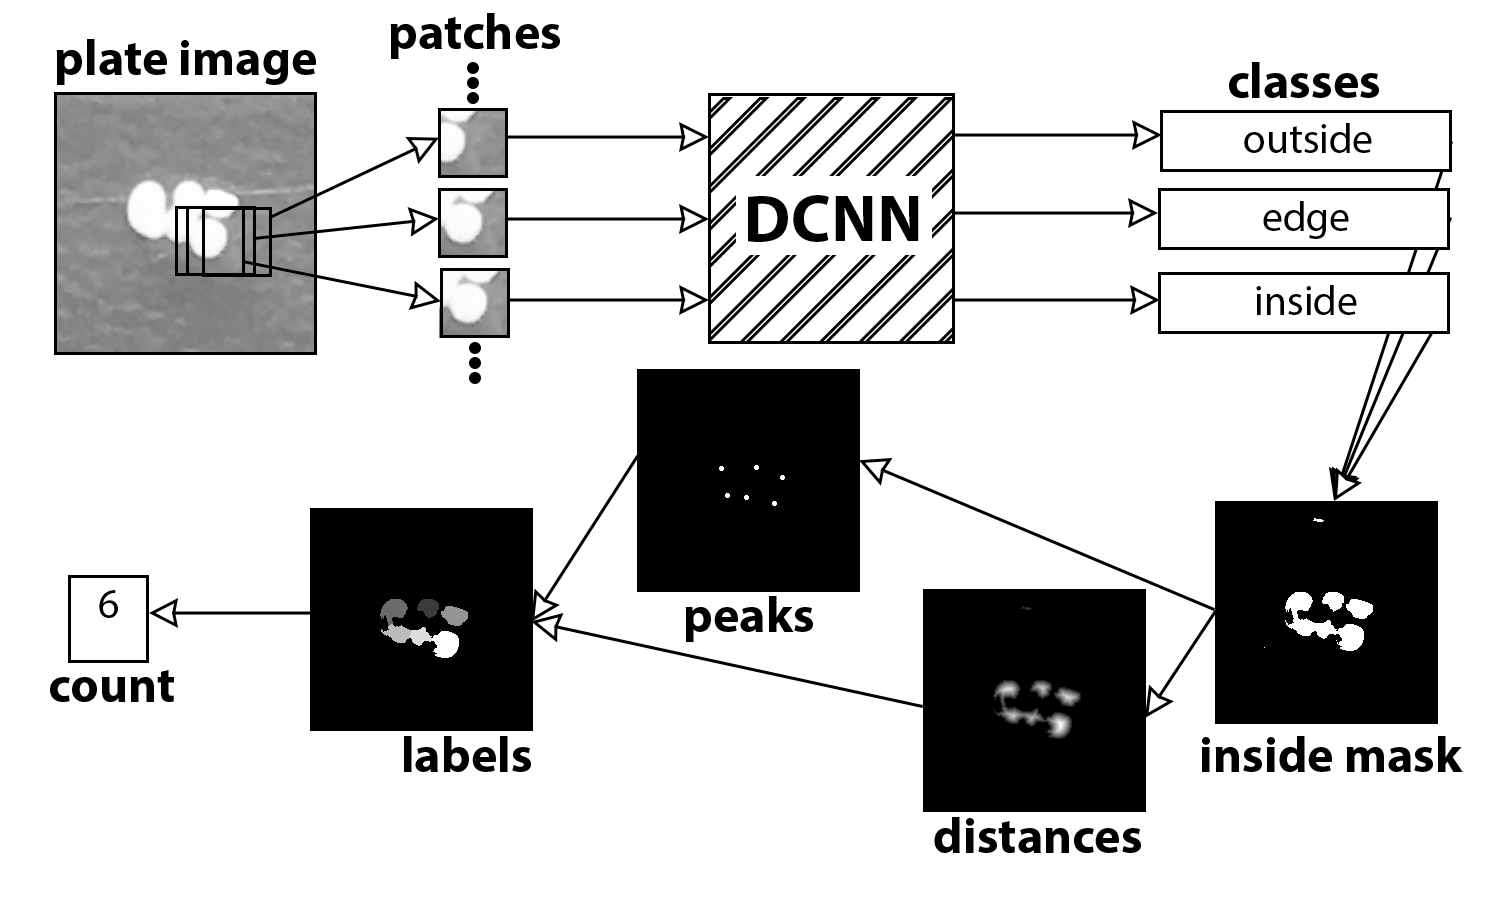
\includegraphics[width=0.7\textwidth]{dcnn_pipeline2}
                \fxnote{Clean this up.}
                \caption{{\bf DCNN Pipeline.} Each pixel of a plate image is classified as either \texttt{inside}, \texttt{edge}, or \texttt{outside} by the DCNN in order to produce a segmentation mask.}
                \label{dcnn_pipeline}
            \end{figure}
        
    
        \paragraph*{Model Overview}
            We present an overview of some key concepts relating to DCNNs below. Specific details on its architecture can be found in \nameref{S1_Text}.
        
            \begin{itemize}
                \item
                    \textit{Neural network.} A neural network is a mathematical object that accepts some inputs and returns some outputs. Neurons in a neural network loosely model biological neurons; they sum up the signals that come in through their input connections, apply a function to the sum, and output the result along their output connections. Connections have strengths which we call weights. Suppose we arranged multiple of these neurons side-by-side in a layer. Mathematically, if the inputs to the network were contained in the vector $x$, the weights of the connections from each input to each neuron were contained in the matrix $W$, and the function the neurons apply were $f$, then the outputs of the neurons would be $f(W \cdot x)$. This situation is depicted in Fig.~\ref{dcnn_neural_network}. Intuitively, by setting up neural networks in this relatively unstructured manner, we give them considerable flexibility to represent a wide class of relationships between their inputs and outputs, depending on the tuning of their weights.
            
                    \begin{figure}[h]
                        \graphicspath{{results/derived/}}
                        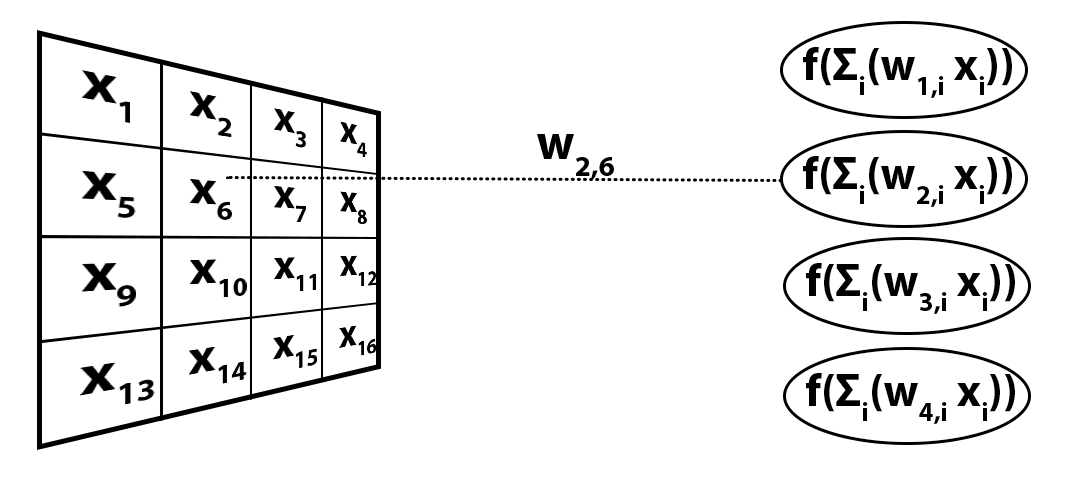
\includegraphics[width=0.7\textwidth]{dcnn_neural_net}
                        \caption{{\bf Neural Network.} Only the connection between input $6$ and neuron $2$ (with weight $w_{2, 6}$) is visualized, but in reality there is a connection between each input and each neuron (each with its own weight $w_{i, j}$).}
                        \label{dcnn_neural_network}
                    \end{figure}
            
                \item
                    \textit{Deep Neural Network.} A deep neural network is a neural network with multiple layers of neurons. In a deep neural network, the inputs of layer $i$ are the outputs of layer $i - 1$. Denoting the matrix of weights coming into layer $i$ as $W_i$, the output of the entire network is the output of the last layer, which is $f(f(\ldots f(x \cdot W_1) \ldots \cdot W_{n-1}) \cdot W_n)$. Intuitively, by stacking these layers, we give the network the power to represent more complex relationships between its inputs and outputs using hierarchical representation.
            
                \item
                    \textit{Convolutional Neural Network.} A convolutional neural network converts the first few layers of the network into convolutional layers which use a different interconnection structure. Instead of connecting each input $i$ to each neuron $j$ using an independent weight $w_{i,j}$, a convolutional layer uses a much smaller number of weights and reuses those same weights on each spatial patch of the input. It is most commonly used when the input is an image. Intuitively, when the input is an image, sharing the same weights across each patch of the image enforces the extraction of the same location-invariant information from each patch of the image, at least in the first few layers of the network.
                
                \item
                    \textit{Neural Network Training.} When a neural network is trained, it is made to produce outputs that, approximately, have some desired relationship with the network's inputs. Training requires a training dataset of both inputs $\{x_1, \ldots, x_n\}$ and their correct outputs $\{y_1, \ldots, y_n\}$, typically containing on the order of at least $100,000$ examples. You feed the network the inputs $x_i$, obtain using the weights $W$ some outputs $\hat{y_i}$ which are interpreted as predicting the correct outputs, and calculate the sum of errors of the predictions, something like $\sum_{i = 1}^n (\hat{y_i} - y_i)^2$. You take the derivative of the error with respect to the weights $\Delta_W (y_i - \hat{y_i})$ and adjust the weights slightly in the direction that reduces this error $W \gets W - 0.01\Delta_W (y_i - \hat{y_i})$. Then you repeat. Over time, the prediction error produced by the weights decreases and the network's outputs become better and better approximations for the correct outputs.
            \end{itemize}

        \paragraph*{Preprocessing}
            The DCNN is trained and validated using a dataset that combines $\texttt{easy\_masked}$ and $\texttt{more\_masked}$. Preprocessing involves a number of steps, notably image normalization as in \cite{Valen} and data augmentation. Image normalization and data augmentation help to ensure the model learns the underlying structure of the problem instead of relying on the brightness or color of the center pixel, since that may vary between experiments, be affected by photographic conditions, or be misleading due to noise.
    
            \begin{enumerate}
                \item
                    We augment the dataset by duplicating each image $10$ times, then randomly modifying the resulting images. With $25\%$ probability, a given image is flipped horizontally or vertically. With $5\%$ probability, a given image gets a random value added to it, gets blurred a random amount, gets random Gaussian noise added to it, gets black and white pixels substituted into it, gets contrast normalized by a random amount, or gets desaturated by a random amount. With $2\%$ probability, a given image gets inverted, gets its hue and saturation changed by a random amount, or gets sharpened by a random amount. An example can be seen in Fig.~\ref{dcnn_augmentation_mutation}.
        
                \begin{figure}[h]
                    \graphicspath{{results/preprocess_masked/figures/original/}}
                    \includegraphics[width=0.25\textwidth,resolution=300]{easy_0_image}
                    \graphicspath{{results/preprocess_masked/figures/augmented/}}
                    \includegraphics[width=0.25\textwidth,resolution=300]{easy_0_image}
                    \includegraphics[width=0.25\textwidth,resolution=300]{easy_1_image}
                    \caption{{\bf Data Augmentation (Mutation).} On the left is an original image. The other two are mutated versions of it.}
                    \label{dcnn_augmentation_mutation}
                \end{figure}
    
            \item
                We then augment the dataset further by duplicating each of the above images $10$ times and rescaling each resulting image by a random factor. An example can be seen in Fig.~\ref{dcnn_augmentation_rescaling}.
    
                \begin{figure}[h]
                    \graphicspath{{results/preprocess_masked/figures/augmented/}}
                    \includegraphics[width=0.25\textwidth,resolution=300]{easy_0_image}
                    \graphicspath{{results/preprocess_masked/figures/resized/}}
                    \includegraphics[width=0.18\textwidth,resolution=300]{easy_0_image}
                    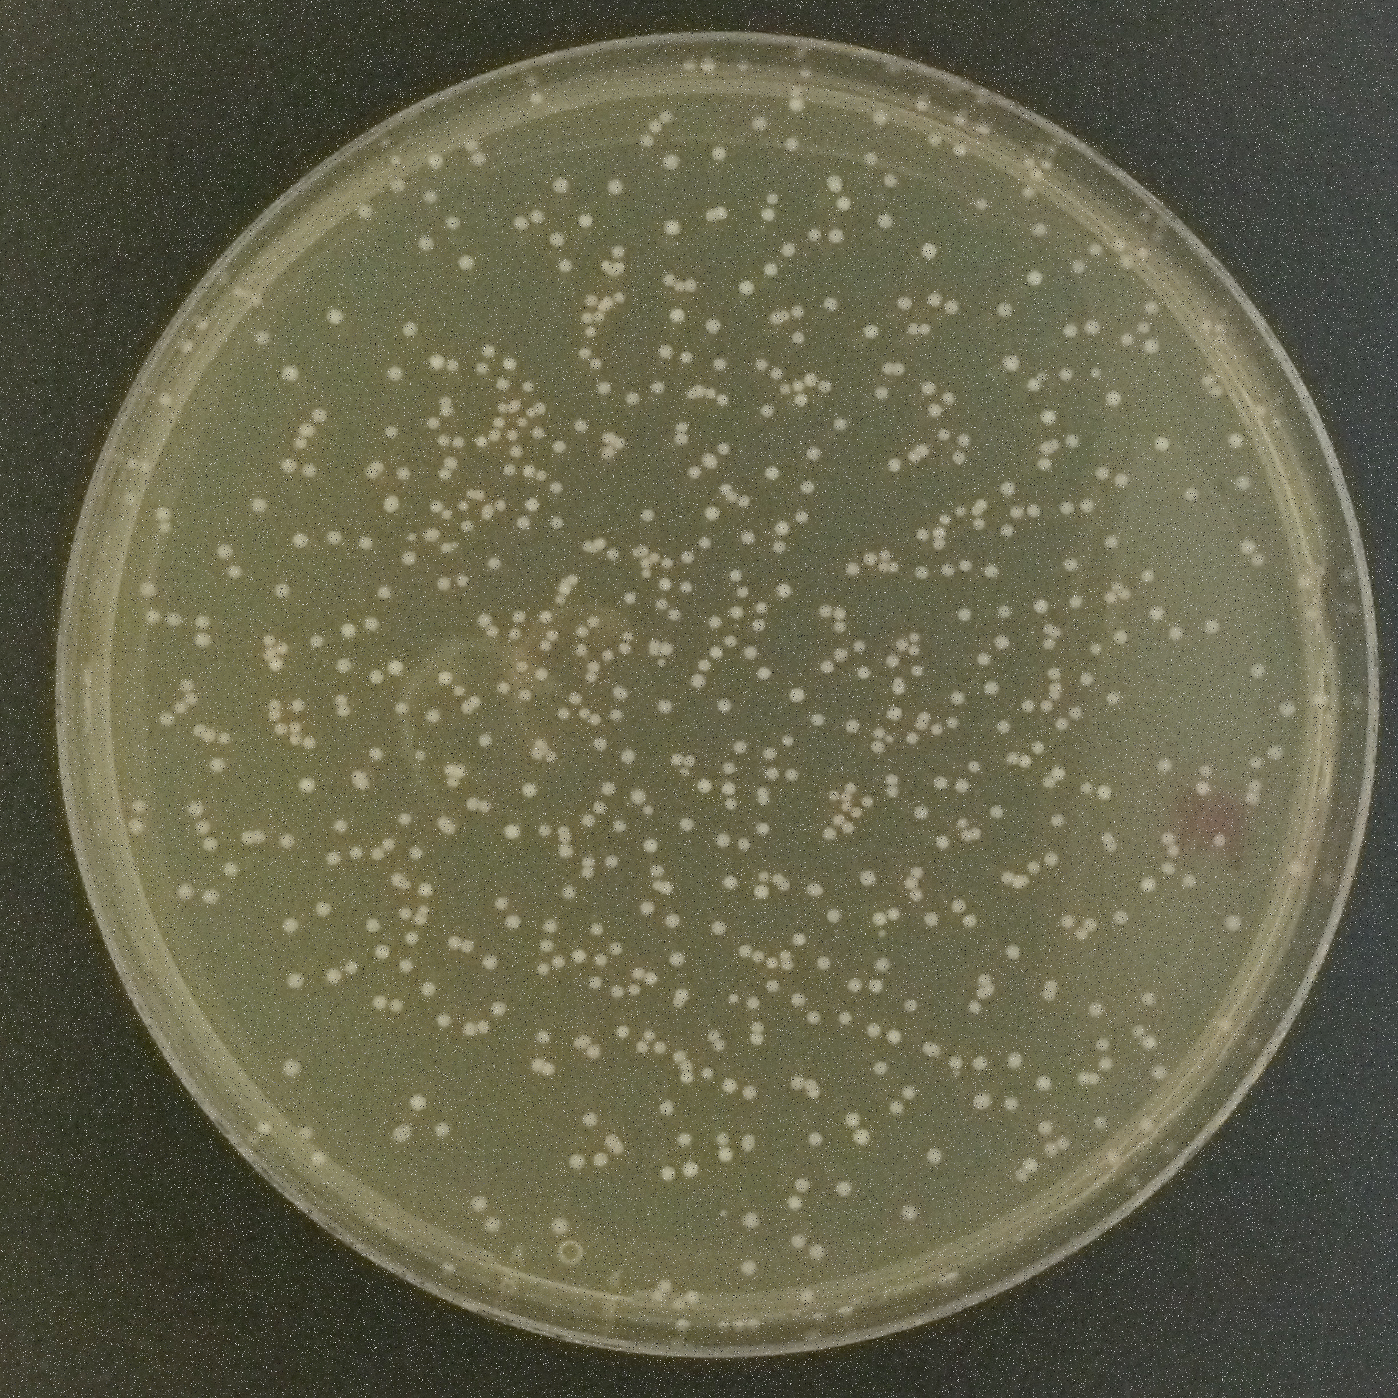
\includegraphics[width=0.32\textwidth,resolution=300]{easy_80_image}
                    \caption{{\bf Data Augmentation (Rescaling). On the left is a mutated image from Fig.~\ref{dcnn_augmentation_mutation}. The other two are rescaled versions of it.}}
                    \label{dcnn_augmentation_rescaling}
                \end{figure}

            \item
                We then normalize the images by dividing out their mean pixel values.
        
            \item
                We extract a total of $1,000,000$ patches of dimensions $61px \times 61px$ from the images. We associate a class -- one of \texttt{inside}, \texttt{edge}, or \texttt{outside} -- with each patch. A patch's class describes its center pixel. For example, if its center pixel is \texttt{inside} a CFU according to the masks, then the patch is considered to be of class \texttt{inside}\fxnote{Add a diagram showing this process.}. The patches are sampled such that all classes are represented equally, even if there are far more \texttt{outside} patches than \texttt{inside} or \texttt{edge}, which is the typical case.
        
            \item
                We normalize the patches by subtracting away their median pixel values.
        
            \item
                We split the dataset into two parts: a training dataset containing $90\%$ of the patches and a validation dataset containing the remaining $10\%$.
    
        \end{enumerate}

     \paragraph*{Training}
        We train the model on $64$-patch batches of the training dataset produced in \nameref{Preprocessing}, looping over the entire dataset a bit more than once\fxnote{Do a training run that loops over the dataset at least twice.} over the course of about $4$ hours. The current version of the model is saved periodically.

     \paragraph*{Validation}
        The training step saves multiple versions of the model, each from a different point during the training process. To determine which version is best, we assess each model's accuracy (proportion of predicted outputs which are correct) on the validation dataset. We choose the model that achieves the highest accuracy to move forward with. Whereas the patches in the training dataset have been used to improve the models, the patches in the validation dataset are until now unseen by the models and therefore may provide a better measure of how they would perform on unseen data.

 

  \subsection*{SVM} \label{ssec:svm}
        \paragraph*{Summary.}
            Our second model is a support vector machine (SVM). In brief, the model takes as input a $61px \times 61px$ image. It outputs a "class", one of \texttt{0-4}, \texttt{5-9}, \texttt{10-19}, or \texttt{20+}. Our goal is to be able to input a $61px \times 61px$ image of an individual well from a $96$-well plate and have the SVM output whether that well contains $0$-$4$, $5$-$9$, $10$-$19$, or $20+$ CFUs.
        
        \paragraph*{Model Overview.}
            We present an overview of some key concepts relating to SVMs below. Specific details on the hyperparameter settings used can be found in \nameref{S2_Text}.
            
            \begin{itemize}
                \item \textit{Support Vector Machine.}
                    A support vector machine (SVM) is a mathematical object that accepts some inputs and returns a class. Assuming there are $d$ inputs, the support vector machine seeks to find the hyperplanes in $\mathbb{R}^d$ that best separate the inputs of each class from the inputs of the other classes. These hyperplanes are defined by some tunable parameters called weights. Mathematically, if the input to the SVM were the vector $x$ and the weights for class $k$ were collected in the vector $w_k$, the SVM would compute a score $w_k \cdot x$ for each class and output the class $k$ with the highest score.
                \item \textit{Support Vector Machine Training.}
                    A SVM is trained using a training dataset of both inputs $\{x_1, \ldots, x_n\}$ and their correct classes $\{y_1, \ldots, y_n\}$. You seek to minimize the sum of squares of the distances by which inputs cross the separating hyperplanes of their correct classes. Since the function to be minimized is quadratic and the constraints are quadratic, the minimum can be found reliably using some standard techniques in quadratic programming.
            \end{itemize}
            
        \paragraph*{Preprocessing}
            We train, validate, and test the SVM using $\texttt{pinned}$.
        
            \begin{enumerate}
                \item We normalize the images by dividing out their mean pixel values.
        
                \item We convert the images into a form that describes their gradients and edges instead of their raw pixels.\fxnote{Add plot.}
        
                \item We discretize the counts by sorting them into the bins $0$-$4$, $5$-$9$, $10$-$19$, and $20+$.
        
                \item We split the dataset into three parts: a training dataset containing $60\%$ of the patches, a validation dataset containing $20\%$, and a test dataset containing the remaining $20\%$.
            \end{enumerate}

        \paragraph*{Training}
            The model has some tunable settings called hyperparameters. We generate $128$ possible assignments of these hyperparameters and train a model for each possible assignment.

        \paragraph*{Validation}
            The training step produces multiple trained models, each with a different assignment of the hyperparameters. To determine which model is best, we assess each model's accuracy on the validation dataset. We choose the model that achieves the highest accuracy to move forward with.

\section*{Results and Discussion}
    \subsection*{DCNN} \label{ssec:dcnn_results}
        \paragraph*{Convergence.}
            As seen in Fig.~\ref{dcnn_convergence}, the DCNN rapidly reaches $85\%$ accuracy after $200$ iterations or about $2$ minutes. After about $4$ hours of training, the accuracy levels out around $89\%$. The accuracy varies more severely in the beginning, before the model begins to stabilize into a local minimum of the error function later on.
            
            \begin{figure}[h]
                \includesvg[svgpath=results/train/19050/,width=0.7\textwidth]{accuracy}
                \caption{{\bf Accuracy Over Training.}}
                \label{dcnn_convergence}
            \end{figure}
        
        \paragraph*{Patch-Based Metrics}
            In both Fig.~\ref{dcnn_convergence} and Fig.~\ref{dcnn_confusion}, the DCNN appears to perform slightly worse on the validation dataset than on the training dataset. This indicates some degree of overfitting, a phenomenon where a model partially memorizes the training dataset which it is learning from. This memorized information reduces the minimization objective (sum of errors on the training dataset), but does not improve the model's performance on unseen data, which is our true goal. The model's performance on the validation dataset is more representative of how it would perform on new data for which we do not have known outputs.
            
            \begin{figure}[h]
                \includesvg[svgpath=results/train/19050/,width=0.4\textwidth]{train_confusion_matrix}
                \includesvg[svgpath=results/train/19050/,width=0.4\textwidth]{valid_confusion_matrix}
                \caption{{\bf Confusion Matrices.} On the left is the DCNN's confusion matrix on a batch of $5,000$ training examples (accuracy $94.72\%$). On the right, on $5,000$ validation examples (accuracy $93.2\%$.}
                \label{dcnn_confusion}
            \end{figure}
        
        \paragraph*{Count-Based Metrics.}             
            Looking at Fig.~\ref{dcnn_plate_counts}, the predicted counts are roughly linearly related to the actual counts, and should be acceptably accurate after multiplication by a compensating factor.
            
            Of particular interest is the DCNN's relative performance on the various datasets. Not surprisingly, it does best with \texttt{easy}. This is to be expected because the \texttt{easy} CFUs are easily counted and since $2/3$ of the plates the DCNN was trained on were from the same batch of plates as \texttt{easy}. However, the DCNN also performs comparably well on \texttt{more}, despite \texttt{more} having CFUs of heterogenous sizes and despite plates from the same batch as \texttt{more} comprising only $1/3$ of the plates the DCNN was trained on. Finally, with a bit more variability, the DCNN also performs well on \texttt{multi}, which is composed of plates from a batch it was never trained on, which are photographed under very poor conditions. This suggests the DCNN is at least somewhat invariant to changes in CFU characteristics and invariant to even large, unfavorable changes in photographic conditions.
            
            \begin{figure}[h]
                \includesvg[svgpath=results/test_countsize100_min1-2/counts/,width=0.7\textwidth]{predicted_vs_actual}
                \caption{{\bf Predicted Counts Versus Actual Counts (Whole Plates). The predicted counts have a strong linear relationship with the actual counts.} Examples from \texttt{easy} appear in yellow, examples from \texttt{multi} appear in purple, and examples from \texttt{more} appear in blue.}
                \label{dcnn_plate_counts}
            \end{figure}

        \paragraph*{Well Counts.} 
            \begin{figure}[h]
                \includesvg[svgpath=results/test_pinned_sampling1-2_min1-8/,width=0.7\textwidth]{predicted_vs_actual}
                \caption{{\bf Predicted Counts Versus Actual Counts (Wells from 96-Well Plates). \_\_\_} \_\_\_}
                \label{dcnn_well_counts}
            \end{figure}
            
            \_\_\_
            
    \subsection*{SVM} \label{ssec:svm_results}
        \paragraph*{Counts.}
            \fillin{long}
                        
            \begin{figure}[h]
                \includesvg[svgpath=results/train_svm/,width=0.4\textwidth]{confusion_matrix}
                \caption{{\bf Predicted Count Ranges Versus Actual Count Ranges. \_\_\_} \_\_\_}
                \label{svm_counts}
            \end{figure}
        
        \paragraph*{Confidence Cutoffs.}            
            SVMs are capable of outputting not only the single most likely class, but a probability for each class. Using this, we can create a metric of confidence. Taking the probability of the most likely class to be $p_1$ and the probability of the second most likely class to be $p_2$, we can consider the confidence of the SVM's prediction to be $p_1 - p_2$. Then, we can consider ignoring predictions below a certain minimum confidence level and instead counting those plates by hand. The result is that we predictions we obtain can be trusted as accurate and the predictions that the SVM cannot make reliably because the plates are too difficult can be passed on to a more appropriately skilled human counter.
            
            \begin{figure}[h]
                \includesvg[svgpath=results/train_svm/,width=0.7\textwidth]{accuracy_vs_cutoff}
                \caption{{\bf Accuracy Versus Confidence Cutoff. The predicted counts have a strong linear relationship with the actual counts.} \_\_\_}
                \label{svm_confidence_accuracy}
            \end{figure}
            
            In doing the above, we trade trade off prediction utilization for higher accuracy of the utilized predictions. By examining the distribution of confidence levels for the SVM's predictions, we can see that a reasonable minimum confidence cutoff might be $0.2$, since only about $10\%$ of predictions do not meet this cutoff. Looking back at Fig.~\ref{svm_confidence_accuracy}, we see that by requiring human intervention for the lowest-confidence $10\%$ of predictions, we would achieve an accuracy of about $0.76$ among the automated predictions, for an accuracy of about $0.78$ overall.\fxnote{Change the confidence metric to "entropy including highest-probability class is lower than $x$".}
            
            \begin{figure}[h]
                \includesvg[svgpath=results/train_svm/,width=0.7\textwidth]{proportion_vs_cutoff}
                \caption{{\bf Predicted Counts Versus Actual Counts. The predicted counts have a strong linear relationship with the actual counts.} \_\_\_}
                \label{svm_confidence_proportion}
            \end{figure}

\section*{Supporting Information}

\subsection*{S1 Text}
\label{S1_Text}
{\bf DCNN Architecture.}  This is a detailed description of the DCNN architecture used in this paper.

\subsection*{S2 Text}
\label{S2_Text}
{\bf SVM Hyperparameters.}  This is a detailed description of the SVM hyperparameter settings considered in this paper.

\section*{Acknowledgments}
\_\_\_

\nolinenumbers

\bibliography{sample}



\end{document}

